\documentclass[12pt,a4paper]{article}
\usepackage[utf8]{inputenc}
\usepackage[english]{babel}
\usepackage[T1]{fontenc}
\usepackage{amsmath}
\usepackage{amsfonts}
\usepackage{amssymb}
\usepackage{subcaption}
\usepackage{makeidx}
\usepackage{graphicx}
\usepackage{fourier}
\usepackage{listings}
\usepackage{color}
\usepackage{hyperref}
\usepackage[left=2cm,right=2cm,top=2cm,bottom=2cm]{geometry}
\author{Vincent Noculak}
\title{Zeeman-Effekt}

\begin{document}

\newpage

\section{Theory}

In physics there are many effects in which light can be scattered by interacting with other particles. In this experiment we will look at the Rayleigh scattering.

Before coming to the theory of Rayleigh scattering we will introduce some other kinds of light scattering.

At the Compton scattering a photon will scatter on a charged particle. By colliding the photon will scatter inelastic, will give some of its energy to the particle and change its direction in some kind of angle

An other kind of scattering is Raman scattering. It can happen, if a photon scatters on an atom or a molecule. Unlike in Rayleigh scattering, the scattered photons have a different wavelength as the incident photons. Due to inelastic scattering the photons can transfer or receive some energy from the molecule/atom they scatter on. This kind of energy difference if specific for the molecule/atom. Raman scattering is of factor of $10^3$ to $10^4$ more unlikely to happen than Rayleigh scattering.

\subsection{Rayleigh scattering}

Rayleigh scattering is the elastic scattering of by particles much smaller than the wavelength of the radiation. Here the incoming light has the same wavelength as the outgoing light.
The scattering can be explained due to that a electromagnetic wave induces a dipole moment at an electron of the atom/molecule in scatters on ($\vec{p}_{ind} = \alpha \cdot \vec{E}$). The electron is now excited, performs as a dipole antenna and emits a photon of the same wavelength as the incident photon.
The cross section of Rayleigh scattering for low frequencies is given by

\begin{equation}
\sigma(\omega) = \sigma_{Th} \frac{\omega^4}{\omega_0^4}
\end{equation}

with $\sigma_{Th} = 0.665 \cdot 10^-24 cm^2$. On this formula we can observe, that Rayleigh scattering is much more likely to happen for light with smaller wavelengths.

This also explains the blue color of the sky. The longer wavelength of the red light gets scattered less than the short wavelength of blue light. Hence from the light of the sun, which gets scattered on the atmosphere of the earth, we see the visible light with the shortest wavelength with the most intensity. Thus the sky appears to be blue.

\subsection{Optical cavity}

An optical cavity is an arrangement of mirrors used to reflect light as often as possible. Depending on how the mirrors are arranged, standing waves can form due to interference. The standing wave, which are possible to form are called the modes of an optical cavity. The components of an optical cavity are ofter a laser, a gas medium it is filled with(in our case the gas medium will play an important role in measuring the Rayleigh scattering) and mirrors. Whether a optical cavity is stable can be calculated with the stability criterion:

\begin{equation}
	0 \leq (1 -  \frac{L}{R_1})(1- \frac{L}{R_2}) \leq 1
\end{equation}

Here $L$ is the length of the resonator and $R_1$ and $R_2$ are the radii of the curvatures of the mirrors. Some examples for optical cavities can be seen in \ref{optical_cavities}.

\begin{figure}[h]
	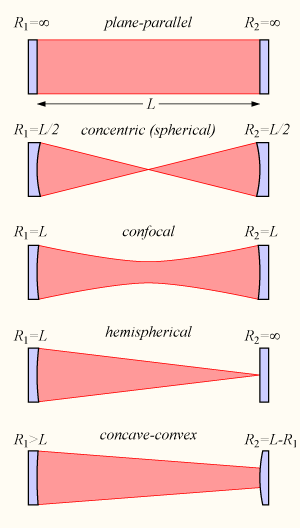
\includegraphics[scale = 0.5]{Optical-cavity1.png}
	\centering
	\caption{Examples for optical cavities, source: \href{https://en.wikipedia.org/wiki/Optical_cavity}{$https://en.wikipedia.org/wiki/Optical_{}cavity$}}
	\label{optical_cavities}
\end{figure}

\subsection{Cavity-Ring-Down Spectroscopy}

Cavity-Ring-Down Spectroscopy is a kind of spectroscopy which uses optical cavities. By filling the resonator with a gaseous sample, the properties of it in scattering or absorbing light can be studied. In the most simple form of the spectroscopy we have 2 highly reflective mirrors and a laser which is in resonance with a cavity mode. Because the mirror only lets a small fraction of the light through, the intensity of the light inside the cavity builds up due to constructive interference. 

Now the laser is turned off and the decay of the light intensity leaking from the cavity is measured. During the decay, the light in the cavity is reflected between the two mirrors. Every time the light hits upon the mirror, a small fraction is able to pass it. Thus the light intesity inside and passing through the mirror will decrease exponentially. If there is a gas inside the cavity which scatters the light, the intensity of the light intensity during the decay process will decrease faster. The decrease of intensity can described by

\begin{equation}
I(t) = I_0 \cdot e^{- \frac{t}{\tau}}
\end{equation}

$\tau$ depends on the wavelength of the laser light

\begin{equation}
\tau (\lambda) = \frac{L}{c (1- R(\lambda) + \beta(\lambda) L)}
\end{equation}

$R(\lambda)$ is the percentage of the light which is reflected by the mirror and $L$ is the length of the resonator. $\beta$ is the scattering coefficient and describes the amount of energy in the laser which gets lost due to the scattering process.

In our experiment we want to determine $\beta$. The scattering process in the cavity will mostly be due to Rayleigh scattering. There is also a small fraction, which will be scatted due to Raman scattering. If we measure one decay process for a vacuum inside the cavity($\beta = 0$, because no scattering is possible) and one with a gas filling up the cavity, we can determine $\beta(\lambda)$ for our laser wavelength with the following formula by measuring the ring-down times $\tau$

\begin{equation}
\beta(\lambda) = \frac{1}{c} (\frac{1}{\tau(\lambda)} - \frac{1}{\tau_0(\lambda)})
\end{equation}

$\tau_0$ is the ring-down time for the cavity with a vacuum inside.

\end{document}